\documentclass[12pt, spanish]{article}


\usepackage{scicite}

\usepackage{times}

\usepackage{graphicx}
\usepackage{caption}
\usepackage{subcaption}

\usepackage{hyperref}

\usepackage{booktabs}



\topmargin 0.0cm
\oddsidemargin 0.2cm
\textwidth 16cm 
\textheight 21cm
\footskip 1.0cm

\newenvironment{sciabstract}{%
\begin{quote} \bf}
{\end{quote}}

\renewcommand\refname{References and Notes}


\newcounter{lastnote}
\newenvironment{scilastnote}{%
\setcounter{lastnote}{\value{enumiv}}%
\addtocounter{lastnote}{+1}%
\begin{list}%
{\arabic{lastnote}.}
{\setlength{\leftmargin}{.22in}}
{\setlength{\labelsep}{.5em}}}
{\end{list}}


% Include your paper's title here

\title{Aprenentatge automàtic aplicat \\ al reconeixement de caràcters en imatges} 


% Place the author information here.  Please hand-code the contact
% information and notecalls; do *not* use \footnote commands.  Let the
% author contact information appear immediately below the author names
% as shown.  We would also prefer that you don't change the type-size
% settings shown here.

\author
{Francesc Aguirre,$^{1}$  Alberto Debernardi$^{2}$\\
\\
\normalsize{$^{1}$Autor: francesc.aguirre@gmail.com}\\
\normalsize{$^{2}$Tutor: adebernardipinos@gmail.com}\\
}

% Include the date command, but leave its argument blank.

\date{23/07/2021}


\begin{document} 
\pagenumbering{gobble}

% Double-space the manuscript.
\baselineskip24pt

\maketitle 

\baselineskip24pt

\begin{center}
	\includegraphics[width=0.15\textwidth]{images/Logo_uab}\par\vspace{1cm}
\end{center}

\clearpage


% Place your abstract within the special {sciabstract} environment.

\begin{sciabstract}
  Aquí anirà el resum en cat, cast, ang.
\end{sciabstract}

\clearpage

\tableofcontents

\clearpage

\pagenumbering{arabic}
%%% (1)
\section{Introducció}

L'estadística és la disciplina que s'encarrega d'analitzar dades per a respondre a preguntes empíriques. A mitjans del segle XX, amb la creació dels dispositius electrònics d'emmagatzematge i l'ajuda de sensors, la quantitat d'informació que es pot recol·lectar ha crescut any rere any. Aquest fet ha donat lloc al naixement de noves disciplines d'anàlisi de dades, tals com la mineria de dades i l'aprenentatge automàtic, més conegut pel seu nom en anglès \textit{machine learning}.

El machine learning és un conjunt de tècniques que dóna als ordinadors l'habilitat d'aprendre de les dades. S'utilitza per a resoldre una gran varietat de problemes predictius complexos en els àmbits d'economia i finances, bioinformàtica, salut, meteorologia, màrqueting, problemes en l'anàlisi i classificació d'imatges, vídeos, àudio... En l'àmbit de l'anàlisi d'imatges hi ha la detecció d'objectes, i més concretament, el reconeixement òptic de caràcters. 

En aquest estudi s'investigarà l'àmbit del reconeixement òptic de caràcters, i com obtenir models predictius competents utilitzant tècniques de machine learning. Per a posar aquests coneixements en pràctica, es resoldrà un problema d'identificació de caràcters irregulars en imatges, tal com la identificació d'escriptura manual o la resolució de \textit{captcha} (és a dir, text en una determinada font que inclou una certa distorsió, precisament per evitar la detecció dels caràcters per part de models més simples, i que són àmpliament utilitzats en internet per evitar l'automatització de determinats processos).


%%% (2)
\section{OCR}

El reconeixement òptic de caràcters OCR (de les sigles en anglès \textit{Optical Character Recognition}) és una aplicació de la intel·ligència artificial, que té com a objectiu detectar i identificar els caràcters que es puguin trobar en una imatge. És una de les àrees més estudiades en l'àmbit de reconeixement de patrons gràcies al gran nombre d'aplicacions pràctiques. Alguns dels problemes que OCR pot ajudar a agilitzar i automatitzar són la digitalització de diaris i llibres antics, la identificació de matrícules, la classificació d'imatges segons el text detectat, i la lectura de dades en paper tals com documentació, correu i enquestes. La digitalització a ordinador de text té moltes més aplicacions, tals com la cerca, edició i emmagatzematge d'informació, traducció, transcripció de text a àudio i NLP (de les sigles en angles \textit{Natural Language Processing}).


% (2.1)
\subsection{Parts tradicionals d'un sistema OCR}

Tradicionalment, un problema típic d'OCR es pot dividir en subtasques en forma de \textit{pipeline} (fetes una darrera l'altre en un ordre concret) que utilitzen tècniques de visió artificial (en anglès \textit{computer vision}), estadístiques i de machine learning. És útil conèixer-les per saber en quin punt del sistema s'està \cite{chaudhuri2017optical}.

\begin{enumerate}
\item Escaneig: És el procés d'escanejar o fotografiar el text \textit{input}. Normalment, al d'escanejar un document s'aplica \textit{thresholding} (binarització) per estalviar memòria i capacitat computacional, que és una tècnica que dicotomitza el color gris de documents en blanc i negre segons un llindar d'intensitat.

\item Segmentació de text: Un cop escanejat el document, típicament el que es vol és obtenir un sol caràcter per utilitzar-lo d'input en el model. La segmentació d'una imatge és la divisió d'aquesta en parts. En aquesta tasca, el que es vol és localitzar el text que ens interessa i ometre gràfics, imatges, logotips... Tot seguit es vol segmentar línies de text, de les línies es segmenten paraules, i de les paraules se segmenten caràcters. En la segmentació ens podem trobar diversos problemes, sobretot si un caràcter està format per diferents parts (i j), si s'està tocant amb algun altre, o s'ha dividit.

\item Preprocessament: Com que el fet d'escanejar o fotografiar una imatge és un procés variable (brillantor, angle...), els caràcters de la imatge segmentada poden contenir soroll, o estar trencats. El preprocessament té com a objectiu eliminar soroll, omplir espais trencats i reduir la grossor dels píxels negres que formen el caràcter. També es normalitzen les dimensions i s'aplicarà una rotació si es detecta inclinació.

\item Segmentació interna: Consisteix a segmentar la imatge del caràcter en seccions més petites, tals com línies i corbes concretes. La intensió és començar a detectar zones amb patrons concrets que facilitin el reconeixement posterior del caràcter.

\item Extracció de variables: A partir de la segmentació interna, se seleccionarà un conjunt de variables que maximitzi el reconeixement amb el nombre menor d'elements. L'objectiu és capturar característiques essencials dels símbols per posteriorment entrenar el model. La extracció de variables més sencilla sería utilitzar la matriu de pixels de la imatge, tot i que utilitzar tantes variables pot provocar problemes de dimensionalitat en molts dels models. Utilitzant extracció de variables, s'utilitzarien característiques que descriguin els caràcters, tals com llargades de segments en regions de la imatge, angles de curvatura...

\item Entrenament i reconeixement: Aplicació de tècniques de reconeixement de patrons per a classificar el caràcter. Aquí és on podem utilitzar tècniques estadístiques i de machine learning per fer la classificació. Alguns models que funcionen força bé són SVM (de l'anglès \textit{support vector machine} i ANN (de l'anglès \textit{artificial neural network}.

\item Reagrupació de caràcters a paraules, paraules a línies, fins a tenir el document complet.
\end{enumerate}

Com es pot veure, la creació d'un sistema OCR tradicional és un procés llarg, amb moltes subtasques que relativament complicades. Els avantatges dels mètodes tradicionals és que donen bons resultats amb mostres petites i són computacionalment eficients. Alguns dels inconvenients és que utilitzen detecció i segmentació de text a partir de tècniques de visió artificial no relacionades amb machine learning, és a dir, no aprenen de les dades. Com que la segmentació no sempre és evident, i les dades poden ser sorolloses, utilitzar aquest tipus de tècniques acostuma a produir errors difícils de solucionar.


% (2.2)
\subsection{Sistema OCR a l'actualitat}

Aquests últims anys, a partir del 2010, el desenvolupament de la branca \textit{deep learning} (aprenentatge profund, una branca de machine learning) a tingut un avanç molt important. La solució en les xarxes neuronals del problema de \textit{vanishing/exploding gradients} i el llançament de noves tecnologies d'alta capacitat computacional tals com noves GPU (de les sigles en anglès \textit{graphics processing unit}), a permès l'entrenament de xarxes neuronals profundes (DNN de les sigles en anglès \textit{deep neural networks}).

Aquest desenvolupament ha donat lloc a nous sistemes OCR basats en xarxes neuronals. La majoria del preprocessament i binarització no és necessari, ja que les xarxes neuronals s'adapten als inputs, podent utilitzar fàcilment els píxels de les imatges. La segmentació de text es pot fer amb tècniques basades en DNN tals com FCN (de les sigles en anglès \textit{Fully Convolutional Networks}), donant millors resultats que amb les tècniques de visió artificial. A més a més, si s'utilitzen RNN (de les sigles en anglès \textit{Recurrent Neural Networks}), no cal segmentar caràcter a caràcter, sinó que es poden utilitzar línies completes de text. Un altre avantatge de les RNN és que poden aprendre de manera natural la llengua utilitzada en l'entrenament. La tendència actual és utilitzar FCN per la segmentació de text en línies, i utilitzar RNN pel seu reconeixement, juntament amb CNN (de les sigles en anglès \textit{Convolutional Neural Networks}) per fer l'extracció de variables \cite{martinek2020building}.

\clearpage
%%% (3)
\section{Problema pràctic}

En aquesta secció es buscaran solucions a un problema pràctic d'OCR. L'objectiu és introduir recursos que ajudin a solucionar un problema del reconeixement de caràcters, i veure quina solució dóna millors resultats. 

Inicialment es buscarà solucionar un problema de reconeixement de caràcters escrits a mà. A primera vista aquest no és un problema fàcil. Hi ha 62 caràcters diferents en l'alfabet anglès, el que implica que a partir d'una imatge, l'algoritme haurà de seleccionar un caràcter entre els 62 disponibles (classes). Si es volgués utilitzar el nostre model per automatitzar completament un procés, es buscaria una precisió propera al 99.5\%. Si es té algú vigilant l'algoritme, llegint que el reconeixement tingui sentit, es pot demanar una precisió més baixa, entre 95\% i 99\%. A més a més, si el que s'analitza són caràcters individuals (sistema tradicional, part de segmentació de text), normalment aquest caràcter forma part d'una paraula, i si aquesta paraula no existeix en el vocabulari, podem fer que el sistema ens avisi (o per exemple, si volem llegir els NIU o id d'alumnes, podem detectar automàticament si existeix el NIU reconegut). Per tant, tot i no aconseguir la precisió més alta, el sistema pot seguir sent útil i no fer errors tan fàcilment. 

% (3.1)
\subsection{Base de dades}

Per a l'elecció de la base de dades, com que s'està experimentant i no es té un objectiu estricte (no s'està participant o ajudant en cap projecte extern al treball), s'ha optat per una base de dades amb una bona quantitat d'exemples i dades ja preprocessades, ja que el preprocessament de dades és una part molt tècnica i metòdica. S'han trobat diferents opcions gratuïtes disponibles en internet, i finalment s'ha utilitzat la base de dades d'imatges de caràcters EMNIST \cite{EMNIST}, derivada de la base de dades d'OCR NIST \cite{watson1992nist}.

La base de dades NIST consisteix en 3669 imatges binaritzades de mostres de formularis fets expressament per testejar mètodes de reconeixement de caràcters (fig:\ref{fig:nist1}). La base de dades també conté els 814,255 caràcters resultants d'aplicar segmentació de text sobre el formulari, en forma d'imatges png de dimensions 128x128 píxels, etiquetades de "0" - "9", de "A" - "Z" i de "a" - "z" en notació hexadecimal. Les imatges segmentades s'han ordenat i etiquetat en diferents organitzacions de carpetes:

\begin{figure}
\centering
\begin{minipage}{.5\textwidth}
  \centering
  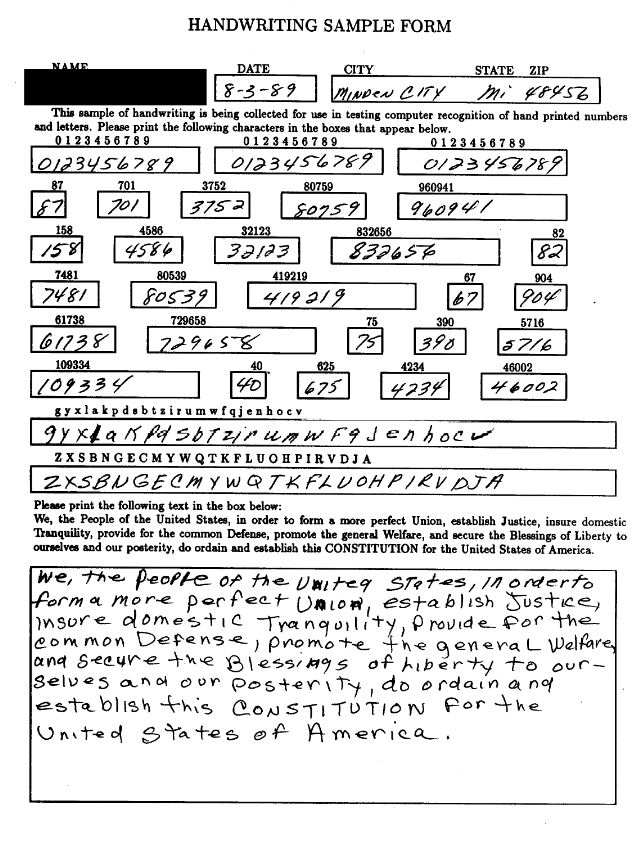
\includegraphics[width=1\linewidth]{images/nist1.jpg}
  \captionof{figure}{Exemple formulari NIST \cite{watson1992nist}}
  \label{fig:nist1}
\end{minipage}%
\begin{minipage}{.5\textwidth}
  \centering
  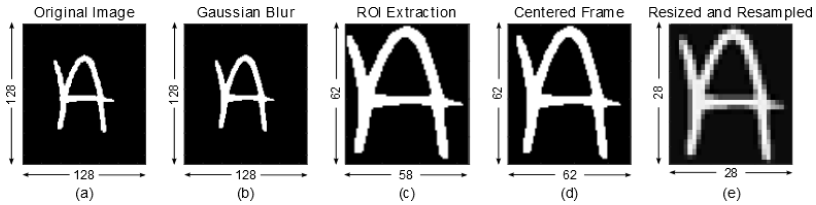
\includegraphics[width=1\linewidth]{images/emnist1.png}
  \captionof{figure}{Transformació d'una imatge NIST a EMNIST \cite{EMNIST}}
  \label{fig:emnist1}
\end{minipage}
\end{figure}

\begin{itemize}
\item Per autor: Els 3669 formularis s'han omplert per persones diferents. Els caràcters segmentats resultants de cada formular-hi s'han agrupat per persona. Aquesta organització no és útil per OCR, sinó per diferenciar tipus d'escriptura segons individus.

\item Per tipus de camp: Les imatges de caràcters s'han dividit pels diferents blocs del formulari: dígits, minúscules, majúscules i text. Seguidament s'han separat per classe de caràcter. Aquest tipus d'organització pot ser molt útil si volem fer models que només continguin un tipus de camp. Per exemple, hi ha tasques, tals com reconeixement de caràcters de formularis, on es demana que s'escrigui només en majúscules, o potser només es volen reconèixer dígits. Entrenar un model amb un nombre de classes possibles reduït serà molt més fàcil que entrenar un model amb 62 classes. A més a més, hi ha classes de caràcters similars de camps diferents ("0", "o", "O"; "I", "l", "1"), que en redimensionar les dimensions de la imatge costaran molt d'identificar. Els diferents camps són fàcils d'identificar en una frase o paraula (majúscules només a l'inici de noms personals o frases, no barrejar números i lletres en una paraula...), però si es barregen les 62 classes a la vegada i s'intenten reconèixer, la dificultat del problema augmentarà, cosa que s'ha de tenir en compte. Aquest també és un dels motius per al que l'ús de RNN per analitzar línies senceres de text funcionen molt bé, perquè aprenen el llenguatge de manera natural, resolent automàticament el problema dels diferents tipus de camps. 

\item Per classe: Les imatges de caràcters estan agrupats en les 62 carpetes de les diferents classes. Amb aquesta organització, tenim el problema de no poder diferenciar entre tipus de camps. 

\item Per fusió de classes: Com que amb l'organització per classe hi ha classes massa similars entre elles, s'ha creat una nova organització ajuntant les classes entre minúscules i majúscules  que s'han considerat més similars (C, I, J, K, L, M, O, P, S, U, V, W, X, Y, Z) i afegint els dígits, fent un total de 47 classes diferents.
\end{itemize}

Els autors també van proposar utilitzar 731,668 imatges de caràcters concretes com a mostra d'entrenament, i 82,587 imatges (amb imatges més desafiants, recol·lectades d'alumnes de secundària) com a mostra de test.

La base de dades EMNIST és el resultat d'agafar les imatges de caràcters de NIST, i aplicar una sèrie de tècniques de preprocessament. Això s'ha fet amb l'objectiu de facilitar l'accés a les dades i estandarditzar el preprocessament de les imatges. D'aquesta manera, els investigadors que vulguin provar nous algoritmes de reconeixement d'imatges poden accedir de manera fàcil a aquestes dades, centrar-se completament en la part d'entrenament  i reconeixement i poder comparar les tècniques des d'una mateixa base. 

El preprocessament (fig:\ref{fig:emnist1}) consisteix en, a partir de les imatges individuals dels caràcters 128x128, primer s'ha aplicat un filtre de desenfocament gaussià per a la reducció de soroll, i tot seguit es retalla la regió d'interès (ROI de les sigles en anglès \textit{region of interest}) deixant de banda files i columnes de píxels blancs, obtenint una imatge d'un caràcter de mida variable. Després se centrarà la imatge de manera que s'evitin píxels negres que toquin els límits de la imatge, afegint files o columnes de píxels blancs, i finalment s'ajustarà la dimensió de la imatge a 28x28 píxels utilitzant un algoritme d'interpolació bicúbic, passant d'una imatge binària a escala grisa (píxels amb intensitat entre 0 i 255)  \cite{EMNIST}.

També s'han aplicat altres passos a la taula de dades, tal com divisió entre mostra d'entrenament i de test, aleatorització de les mostres i la creació d'altres organitzacions de carpetes. S'ha afegit l'organització balancejada, que és similar a l'organització per fusió de classes, però on cada classe té el mateix nombre d'exemples que la resta, resultant en una mostra de 131,600 exemples i 47 classes, només dígits amb 280,000 exemples i 10 classes, només lletres amb 145,600 exemples i 26 classes i la base de dades MNIST (dígits d'alumnes de secundària) amb 70,000 exemples i 10 classes. L'organització que s'ha utilitzat en aquest projecte és la balancejada majoritàriament, perquè és la que proporciona les prediccions més justes (amb menys biaix), tot i que en contrapartida s'estan sacrificant molts exemples. Puntualment pot ser interessant experimentar amb l'organització per fusió de classes a l'entrenar els models, per veure si augmentar la mida de les dades fa millorar les prediccions. Altres opcions interessants són l'organització per només dígits o només lletres.


% (3.2)
\subsection{Descriptius i visualitzacions}

La variable dependent d'aquest problema és la classe de la imatge. Sobre aquesta variable, és interessant veure el nombre d'exemples (freqüència absoluta) que hi ha per classe, per saber si la variable està balancejada, i com es distribueix. Però com que podem tenir fins a 62 classes diferents, és massa tediós analitzar classe per classe, per tant s'han calculat descriptius del nombre d'exemples per classe, tals com la mitjana, desviació estàndard, mínim i màxim per tenir una idea general d'aquesta variable, segons l'organització (base de dades) utilitzada (tab:\ref{tab:taula1}). El primer que crida l'atenció és que l'organització per fusió, que és la que té més exemples, té una alta variabilitat d'exemples entre classes, anant des de 3,000 fins a 38,000 exemples. D'aquesta organització, el nombre d'exemples de dígits és més elevat que la resta i té poca variabilitat entre si, mentre que el nombre d'exemples de lletres és menor i amb més variabilitat. Les organitzacions adicionals de la base de dades EMNIST balancejades, dígits i lletres, arreglen el problema del desbalanceig de classes, tot i que es redueixen considerablement el nombre d'exemples. 

\begin{table}[hbt!]
\centering
\begin{tabular}{lcccccc}  
\toprule
                            & Fusió & Fusió dígits & Fusió lletres & Balancejat & Dígits & Lletres \\  
\midrule
nombre exemples    & 697,932 & 345,426  & 352,506 & 112,800 & 240,000 & 124,800 \\
nombre classes        & 47         & 10          & 37         & 47        & 10          & 26      \\
Mitjana                   & 14,849   & 34,542    & 9527     & 2,400    & 24,000    & 4,800 \\
Desviació estandard  & 11,743   & 1,713      & 6423    & 0           & 0            & 0       \\
Mínim                     & 2,534      & 31,280   & 2534    & 2,400      & 24,000   & 4,800 \\
Màxim                    & 38,304    & 38,304   & 27664   & 2,400      & 24,000   & 4,800 \\
\bottomrule
\end{tabular}
\captionof{table}{Descriptius sobre el nombre d'exemples per classe. Es descriu la mitjana i desviació de la freqüència absoluta d'exemples per classe, seguit de la freqüència mínima i la màxima, segons les diferents organitzacions de la base de dades EMNIST.}
\label{tab:taula1}
\end{table}


Passant a les variables explicatives, quan es treballa amb imatges és difícil extreure idees de les variables independents, perquè són molts píxels en diferents intensitats. Per fer-se una idea de quines imatges ens podem trobar,  pot ajudar visualitzar alguns exemples de la base de dades (fig:\ref{fig:sample_random}).

\begin{figure}[hbt!]
\centering
	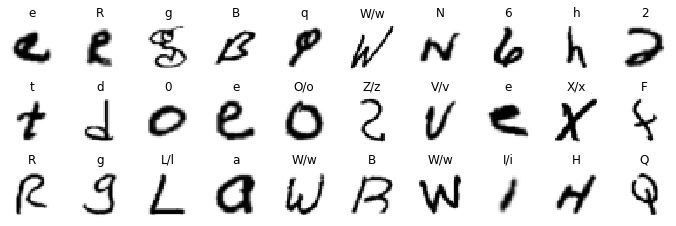
\includegraphics[width=1\textwidth]{images/samples_balanced.png}
	\captionof{figure}{Submostra aleatòria de 30 exemples de les dades EMNIST amb organització balancejada.}
	\label{fig:sample_random}
\end{figure}

De la figura \ref{fig:sample_random}, com que s'han utilitzat les dades amb organització balancejada, es pot comprovar que algunes  de les classes s'han ajuntat en una sola ("W/w", "O/o"...). També podem fer-nos una primera idea de la dificultat del problema. La majoria d'exemples es poden reconèixer a primer cop d'ull, però algun exemple com la segona fila sisena columna amb etiqueta "Z/z", sense cap altre context, una persona ho podria llegir com a "2".

Per fer-nos una idea de com són els exemples per classe, s'han visualitzat alguns exemples per classe (Annex fig:\ref{fig:sample_by_label}). Aquesta figura ajuda a veure similituds i diferències entre classes. Es pot veure que a simple vista i sense cap altre context, les imatges amb classes ["1", "I/i", "L/l"] són molt similars, el mateix per les classes ["0", "O/o"], ["q" i "9"], ["h", "n"] i potser ["a", "2"]. També podem veure que hi ha alguns errors d'etiquetació o de formulari, o potser s'ha perdut qualitat d'imatge a causa del preprocessament, però de la classe "G" la columna 6 sembla una "S/s", de la classe "H" la columna 2 sembla una "W/w", de la classe "g" la columna 1 sembla "a" i de la classe "q" la columna 7 sembla "8". Per tant, estem en un problema de classificació que fins i tot a ull humà i sense cap altre context, seria difícil aconseguir una precisió propera al 95\%. També s'ha calculat la intensitat de pixel mitjà per cada classe i s'ha projectat en una imatge, el que dona una idea força clara de la imatge mitjana en cada classe, o les regions de la imatge en que el caràcter s'acostuma a veure (Annex fig:\ref{fig:samples_by_mean}).

Una altre idea per a veure aquestes similituds i diferències entre classes, és aplicar tècniques no supervisades de reducció de dimensions. Una tècnica que acostuma a donar bons resultats per a visualitzacions de clusters d'espais d'alta dimensió és el t-Distributed Stochastic Neighbor Embedding (t-SNE). T-SNE és una tècnica de reducció de dimensions no lineal de tipus \textit{manifold learning}, que consisteix en modelar cada exemple d'alta dimensió en un punt de 2-3 dimensions a partir de probabilitats conjuntes, de manera que exemples similars són més propers que exemples diferents, el que ho fa un mètode perfecte per visualitzar clusters.

Com que tenim una mostra d'entrenament i dimensions grans (101,520 exemples, 784 variables), per a reduïr soroll i accelerar temps computacional és bona idea aplicar un segon mètode de reducció de dimensions abans d'utilitzar t-SNE. S'ha utilitzat components principals per reduïr la dimensió fins a un 95\% de la variància explicada (113 variables), i tot seguit s'ha aplicat t-SNE per a reduïr la dimensió a 2 variables. Tot i que és difícil mapejar 47 classes diferents, l'algoritme t-SNE ha funcionat força bé (Annex fig:\ref{fig:pca_tsne}). En la figura \ref{fig:pca_tsne} es mostren les 2 dimensions resultants, on cada color és una classe. En la regió sud es veuen una serie de clusters ben separats ["u", "w", "N", "m", "H"]. Seguint el sentit de les agulles del rellotge en la regió sud-oest es veu un cluster de ["0", "O"], juntament amb els clusters ["D" i Q"], indicant que per aquesta zona els caracter són arrodonits. A l'oest hi ha els clusters ["G", "C", "e", "6"]. Al nord-oest es veuen els ["8", "3", "5"]. A la regió nord, nord-est hi ha caràcters formats per un segment central vertical, tal com el gran cluster ["1", "l", "I"], juntament amb els clusters ["T", "J", "7", "f"]. Finalment a la regió est hi ha caràcters formats per més d'una línia diagonal al plà ["y", "V", "X"]. 

Si volem veure de mes aprop algunes de les classes més sobreposades tals com ["0", "O/o", "Q", "D"] o ["I/i", "L/l", "1"], podem entrenar un t-SNE amb aquestes classes per separat (fig:\ref{fig:tsne2}). Com era d'esperar, tot i que una part de les imatges de les classes "D" i "Q" es diferencien de la resta, tant "O/o" com "0" es barregen en el mateix cluster. Similarment, tot i que algunes "L/l" i "I/i" es distingueixen de la resta (segurament majuscules "L", o "i"), les classes "L/l", "1" i "I/i" són difícils de distingir. Això fa veure que seran necessaris models molt complexos si es vol arribar a distingir entre aquestes classes, o s'haurà de recorre a altres alternatives tals com modelar números i lletres per separatm modelitzar imatges segmentades per línies o aconseguir informació de context adicional (en quina posició s'està de la paraula, paraula després d'un punt...).

\begin{figure}%[hbt!]
\centering
\begin{minipage}{.5\textwidth}
  \centering
  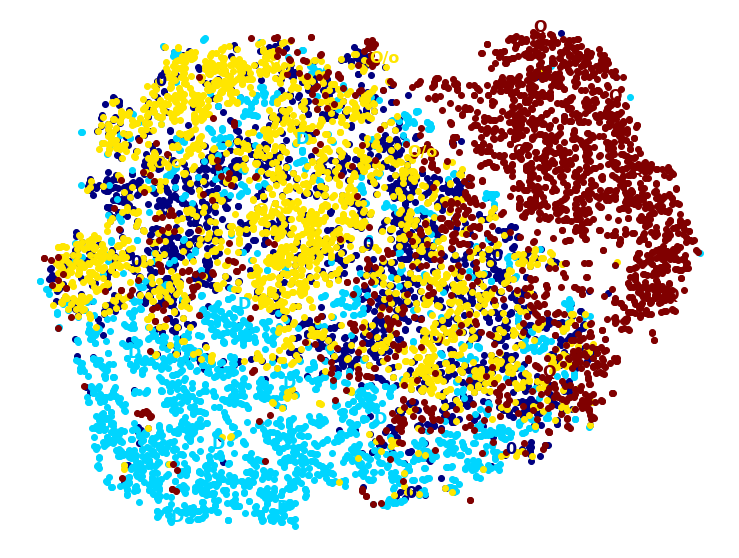
\includegraphics[width=.95\linewidth]{images/tsne_sub1.png}
\end{minipage}%
\begin{minipage}{.5\textwidth}
  \centering
  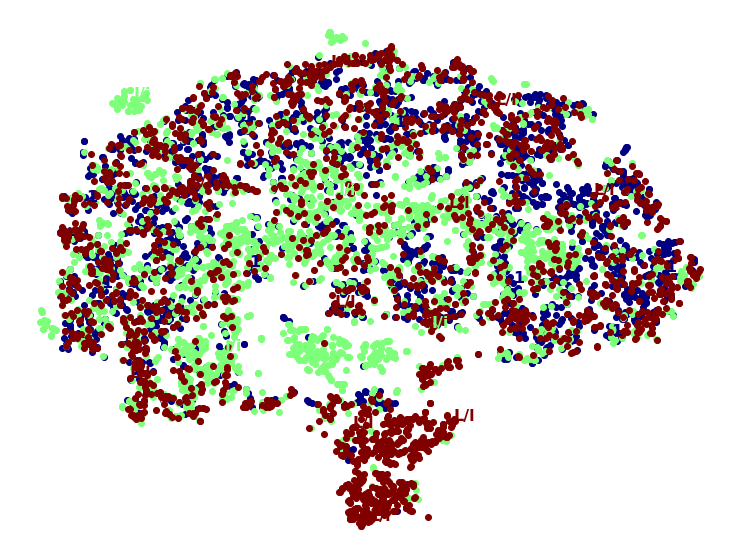
\includegraphics[width=.95\linewidth]{images/tsne_sub2.png}
\end{minipage}%
  \captionof{figure}{t-SNE sobre les dades EMNIST balancejades. A la figura de l'esquerra s'han utilitzat les classes ["0", "O/o", "Q", "D"]. A la figura de la dreta s'han utilitzat les classes ["I/i", "L/l", "1"].}
  \label{fig:tsne2}
\end{figure}


% (3.3)
\subsection{Preprocessament}

Abans d'entrenar els models, és important haver fet el preprocessament necessari. Normalment es té una mostra d'entrenament amb la que s'entrenaran els models i una mostra de testeig per veure com generalitzen els models finalment. La mostra de testeig no es tocarà mai durant el procés d'entrenament, per tant s'han de tenir alternatives per a validar els models i refinament d'hyperparàmetres, tals com una mostra de validació o l'ús de tècniques tals com \textit{cross validation}. L'alternativa de la mostra de validació és atractiva quan es tenen models computacionalment difícils d'entrenar i una quantitat d'exemples raonable, per tant s'ha fet una petita mostra de validació amb el 10\% dels exemples de la mostra d'entrenament, resultant una mostra d'entrenament amb 101,520 exemples (77.1\%), una mostra de validació amb 11,280 exemples (8.6\%) i una mostra de test amb 18,800 exemples (14.3\%) en l'organització balancejada.

En aprenentatge supervisat, també és típic l'ús d'algoritmes d'optimització online tals com GD, SGD \textit{de les sigles en anglès \textit{Stochastic Gradient Descent}}, que fan una estimació dels paràmetres d'un model de manera iterativa. Aquests algoritmes requereixen una mostra aleatòria per arribar a una bona optimització, per això és important aleatorietzar l'ordre dels exemples. El conjunt de dades EMNIST ja ve distribuït aleatoriament. 

Un últim pas de preprocessament que requereixen alguns algoritmes és l'escalament de variables. Si els inputs tenen rangs o distribucions molt diferents, és important estandaritzar o normalitzar les variables. També dependra del tipus d'algoritme que s'utilitzi, però per norma general, si necessitem que els inputs tinguin un rang fixat es normalitzaran les dades, i si les variables ténen outliers importants (valors extrems) és més recomanable estandaritzar.

Altres tècniques de preprocessament poden ajudar a millorar i regularitzar els models. Una opció és utilitzar \textit{data augmentation} en imatges a partir de rotacions, donant la volta, reescalament de dimensions, canvis de llum, contrast i deformació elàstica. Hi ha models que no funcionen bé quan en nombre de variables i exemples és molt gran, de manera que és recomanable aplicar el pas d'extracció de variables. Altres opcions són aplicar tècniques de reducció de dimensions tals com components principals o l'ús d'\textit{autoencoders}, per en alguns casos accelerar el temps d'entrenament i reduir el soroll, tot i que normalment es perdrà precisió.

% (3.4)
\subsection{Models d'aprenentatge automàtic}

% X Regressió logistica multinomial
% X Lineal SVM
% X Kernel SVM (least squares SVM?)
% X Random Forest
% X ANN
% X CNN
% LVQ
% Naive Bayes classifier
% LDA

En aquesta part del treball s'han de buscar models candidats. En principi, qualsevol model de classificació pot ser utilitzat, però n'hi haura que classificaran millor i més eficientment les dades EMNIST. Aquesta és una tasca de classificació multiclasse, però encara que un model sigui per naturalesa de classificació binaria (ex: model logistic, SVM), es poden utilitzar estrategies com OvO (\textit{one versus one}) o OvA (\textit{one versus all}) i fer-los servir com a classificació multiclasse. 

Primer s'han entrenat tots els models sense un tuneig d'hyperparàmetres excesiu i amb una mostra reduïda, i s'han avaluat tant sobre la mostra d'entrenament com sobre la de validació, per comprobar l'\textit{overfitting}/\textit{underfitting} dels models (tab:\ref{tab:taula2}). A partir d'aquí s'han triat els models que han semblat tenir major potencial, s'han tunejaran els hyperparàmetres i s'han entrenat els models finals. 

\subsubsection{Regressió logística multinomial}

[TODO explicació general]

Abans d'entrenar el model, és necessari reduïr les dimensions amb alguna tècnica com PCA, perquè en càs contrari és complica trobar una solució optima fàcilment (sense gastar recursos computacionals). Amb 113 components s'ha conservant el 95\% de la variància explicada, i s'han escalat els inputs. El model ha estat entrenat amb una submostra de 10,000 exemples, i s'ha utilitzat l'optimitzador \textit{limited-memory BFGS} amb regularització l2 i l'hyperparàmetre C = 1, amb una tolerancia de 0.001 i 500 iteracions màximes.

\subsubsection{Lineal SVM}

[TODO explicació general]

Per entrenar el lineal SVM, s'ha utilitzat una submostra d'entrenament de 10,000 exemples. Per a l'optimització s'ha utilitzat SGD (de les sigles en anglès \textit{stochastic gradient descent}) amb regularització l2 i hyperparàmetre factor de regularització, alpha = 1e-4 (com més alt, més regularització), amb una tolerancia de 5e-3 i 500 iteracions màximes.

\subsubsection{Kernel SVM}

[TODO explicació general]

En aquest cas, per entrenar el Kernel SVM s'ha utilitzat una submostra d'entrenament de 5,000 exemples. Això és degut a que el temps computacional al entrenar Kernel SVM és entre $O(n^2 p)$  i $O(n^3 p)$, de manera que si augmentem el nombre d'exemples sense cura l'entrenament podria durar hores. Una alternativa és utilitzar SGD utilitzant una aproximació \textit{Nystroem} a priori. S'ha utilitzat un kernel gaussià RBF (de les sigles en anglès \textit{radial basis function}), amb regularització l2 i hyperparàmetre C = 1, amb una tolerància de 0.001 i 500 iteracions màximes. 

\subsubsection{Random Forest}

[TODO explicació general]

Per entrenar el random forest s'ha utilitzat una submostra d'entrenament de 10,000 exemples, utilitzant 100 arbres sense restriccions i amb mostres \textit{bootstrap}. 

\subsubsection{ANN}

[TODO explicació general]

Per entrenar la xarxa neuronal o MLP (de les sigles en anglès multilayer perceptron), s'ha utilitzat una estructura seqüencial amb tres capes ocultes completament conectades \ref{fig:nn_estructure}. La primera capa d'inputs és la imatge de dimensions 28x28, la segona capa és de preprocessament, aplanant les dimensions a 784 neurones input, la següent és la primera capa oculta amb 400 neurones, la segona capa oculta té 200 neurones, la tercera té 100 neurones, i finalment la última capa és d'outputs. Les capes ocultes tenen funció d'activació relu, i la última capa té funció d'activació \textit{softmax}. 




\subsubsection{CNN}

[TODO explicació general]










% (3.5)
\subsection{Resultats}

\begin{table}[hbt!]
\centering
\begin{tabular}{lcccc}  
\toprule
                                              & N         & T (s)  & Acc train (\%) & Acc val (\%) \\  
\midrule
Regressió logística multinomial  & 10,000 & 5   & 77.0        & 63.4 \\
Lineal SVM                              & 10,000 & 41  & 73.3       & 61.8  \\
Lineal SVM amb PCA                & 10,000 & 5    & 70.4       & 56.7  \\
Kernel SVM                             & 5,000   & 5    & 89.0       & 68.8  \\
Kernel SVM amb PCA               & 5,000   & 3    & 94.5       & 64.8  \\
Random Forest                        & 10,000 & 10  & 100.0     & 72.3 \\
Random Forest amb PCA          & 10,000 & 14  & 100.0     & 66.2  \\
ANN 					     & 101,520 * 5 & 42 & 80.3 & 80.2  \\
ANN amb PCA                         & 101,520 * 5 & 20 & 59.3 & 55.4 \\
CNN					     & 10,000 * 5   & 158 & 75.3 & 80.4 \\
\bottomrule
\end{tabular}
\captionof{table}{Models amb el seu rendiment (precisió). Les columnes són el nom del model, el nombre d'exemples en la mostra de d'entrenament (* epoch), els segons a entrenar el model, la precisió sobre la mostra d'entrenament i la precisió sobre la mostra de validació.}
\label{tab:taula2}
\end{table}

A la taula (tab:\ref{tab:taula2}) s'han obtingut els resultats dels primers models plantejats. Els models amb la major precisió en la mostra de validació són la CNN, la ANN, el random forest i el kernel SVM. Especialment les xarxes neuronals, tenen una precisió major en la mostra de validació que en la mostra d'entrenament, el que indica que els models estan \textit{underfitting}, i si utilitzem la mostra d'entrenament completa, augmentem el nombre d'\textit{epochs} o augmentem la complexitat de la xarxa, podriem obtenir millors resultats. Per el contrari, el random forest i el kernel SVM estan overfitting, si augmentem els hyperparàmetres de regularització és possible que augmenti la precisió en noves dades. El següent pas és afinar els models retocant els hyperparàmetres i acabant d'entrenar els models.






% (4)
\section{Conclusions}

[TODO]

Parlar sobre que queda per explorar:

- Reducció de dimensions utilitzant autoencoders-

% Annex
\clearpage
\appendix \label{sec:A}
\section{Gràfics}


\begin{figure}[hbt!]
\centering
\begin{minipage}{.33\textwidth}
  \centering
  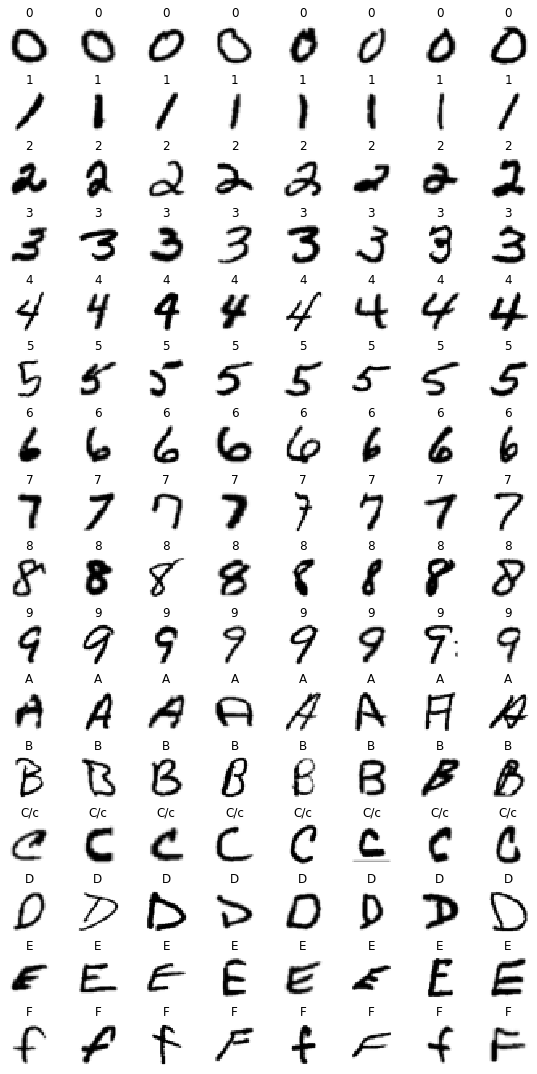
\includegraphics[width=.95\linewidth]{images/samples_by_label1.png}
\end{minipage}%
\begin{minipage}{.33\textwidth}
  \centering
  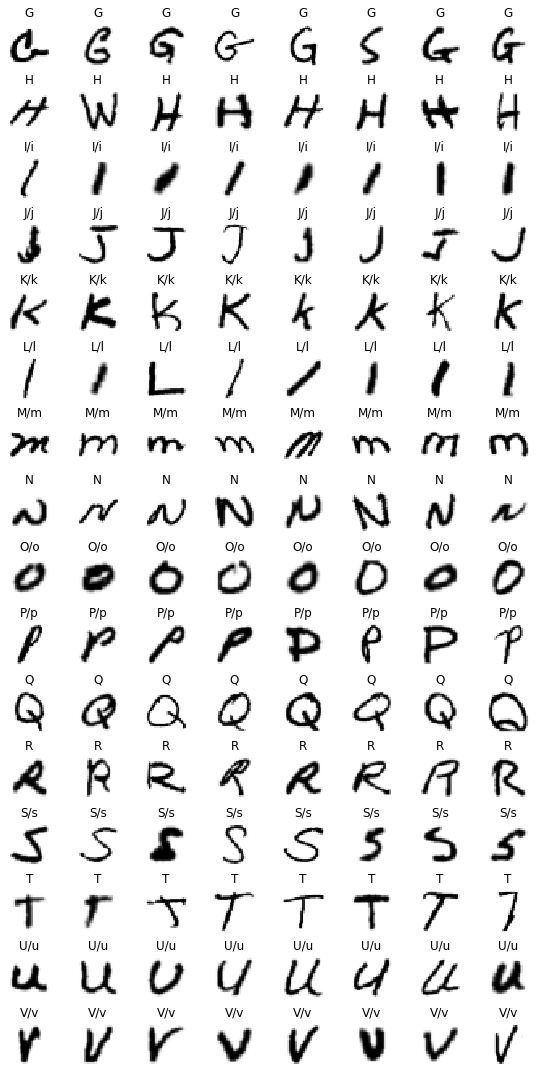
\includegraphics[width=.95\linewidth]{images/samples_by_label2.png}
\end{minipage}%
\begin{minipage}{.33\textwidth}
  \centering
  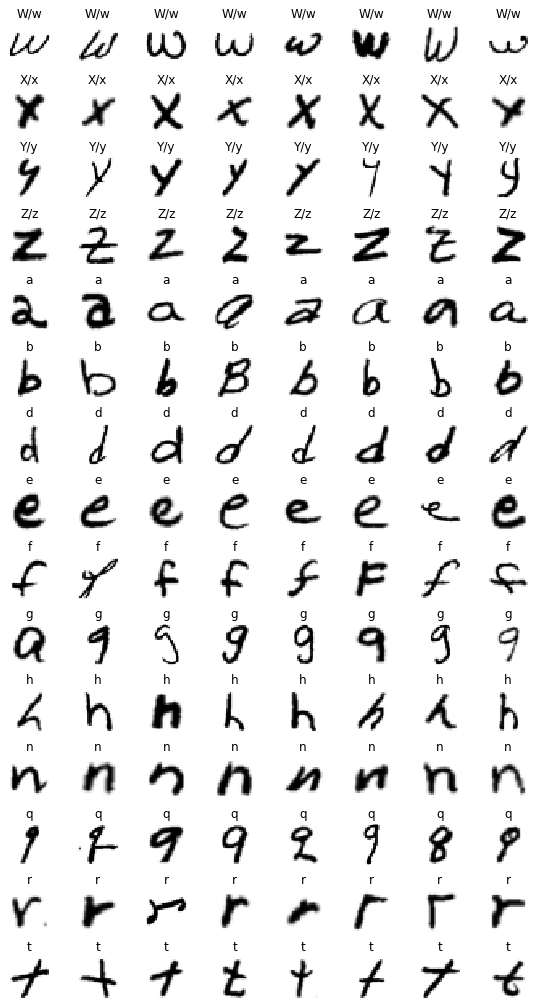
\includegraphics[width=.95\linewidth]{images/samples_by_label3.png}
\end{minipage}%
  \captionof{figure}{Submostres aleatòries de la base de dades EMNIST amb organització balancejada. 8 exemples per classe.}
  \label{fig:sample_by_label}
\end{figure}

%%%

\begin{figure}[hbt!]
\centering
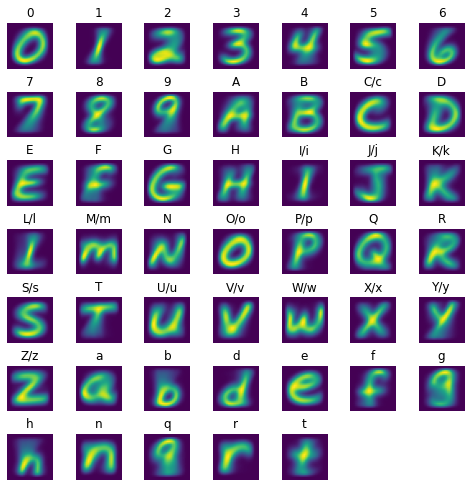
\includegraphics[width = 1\linewidth]{images/samples_by_mean.png}
\captionof{figure}{Intensitat de pixel mitjà per classe.}
\label{fig:samples_by_mean}
\end{figure}

%%%

\begin{figure}[hbt!]
\centering
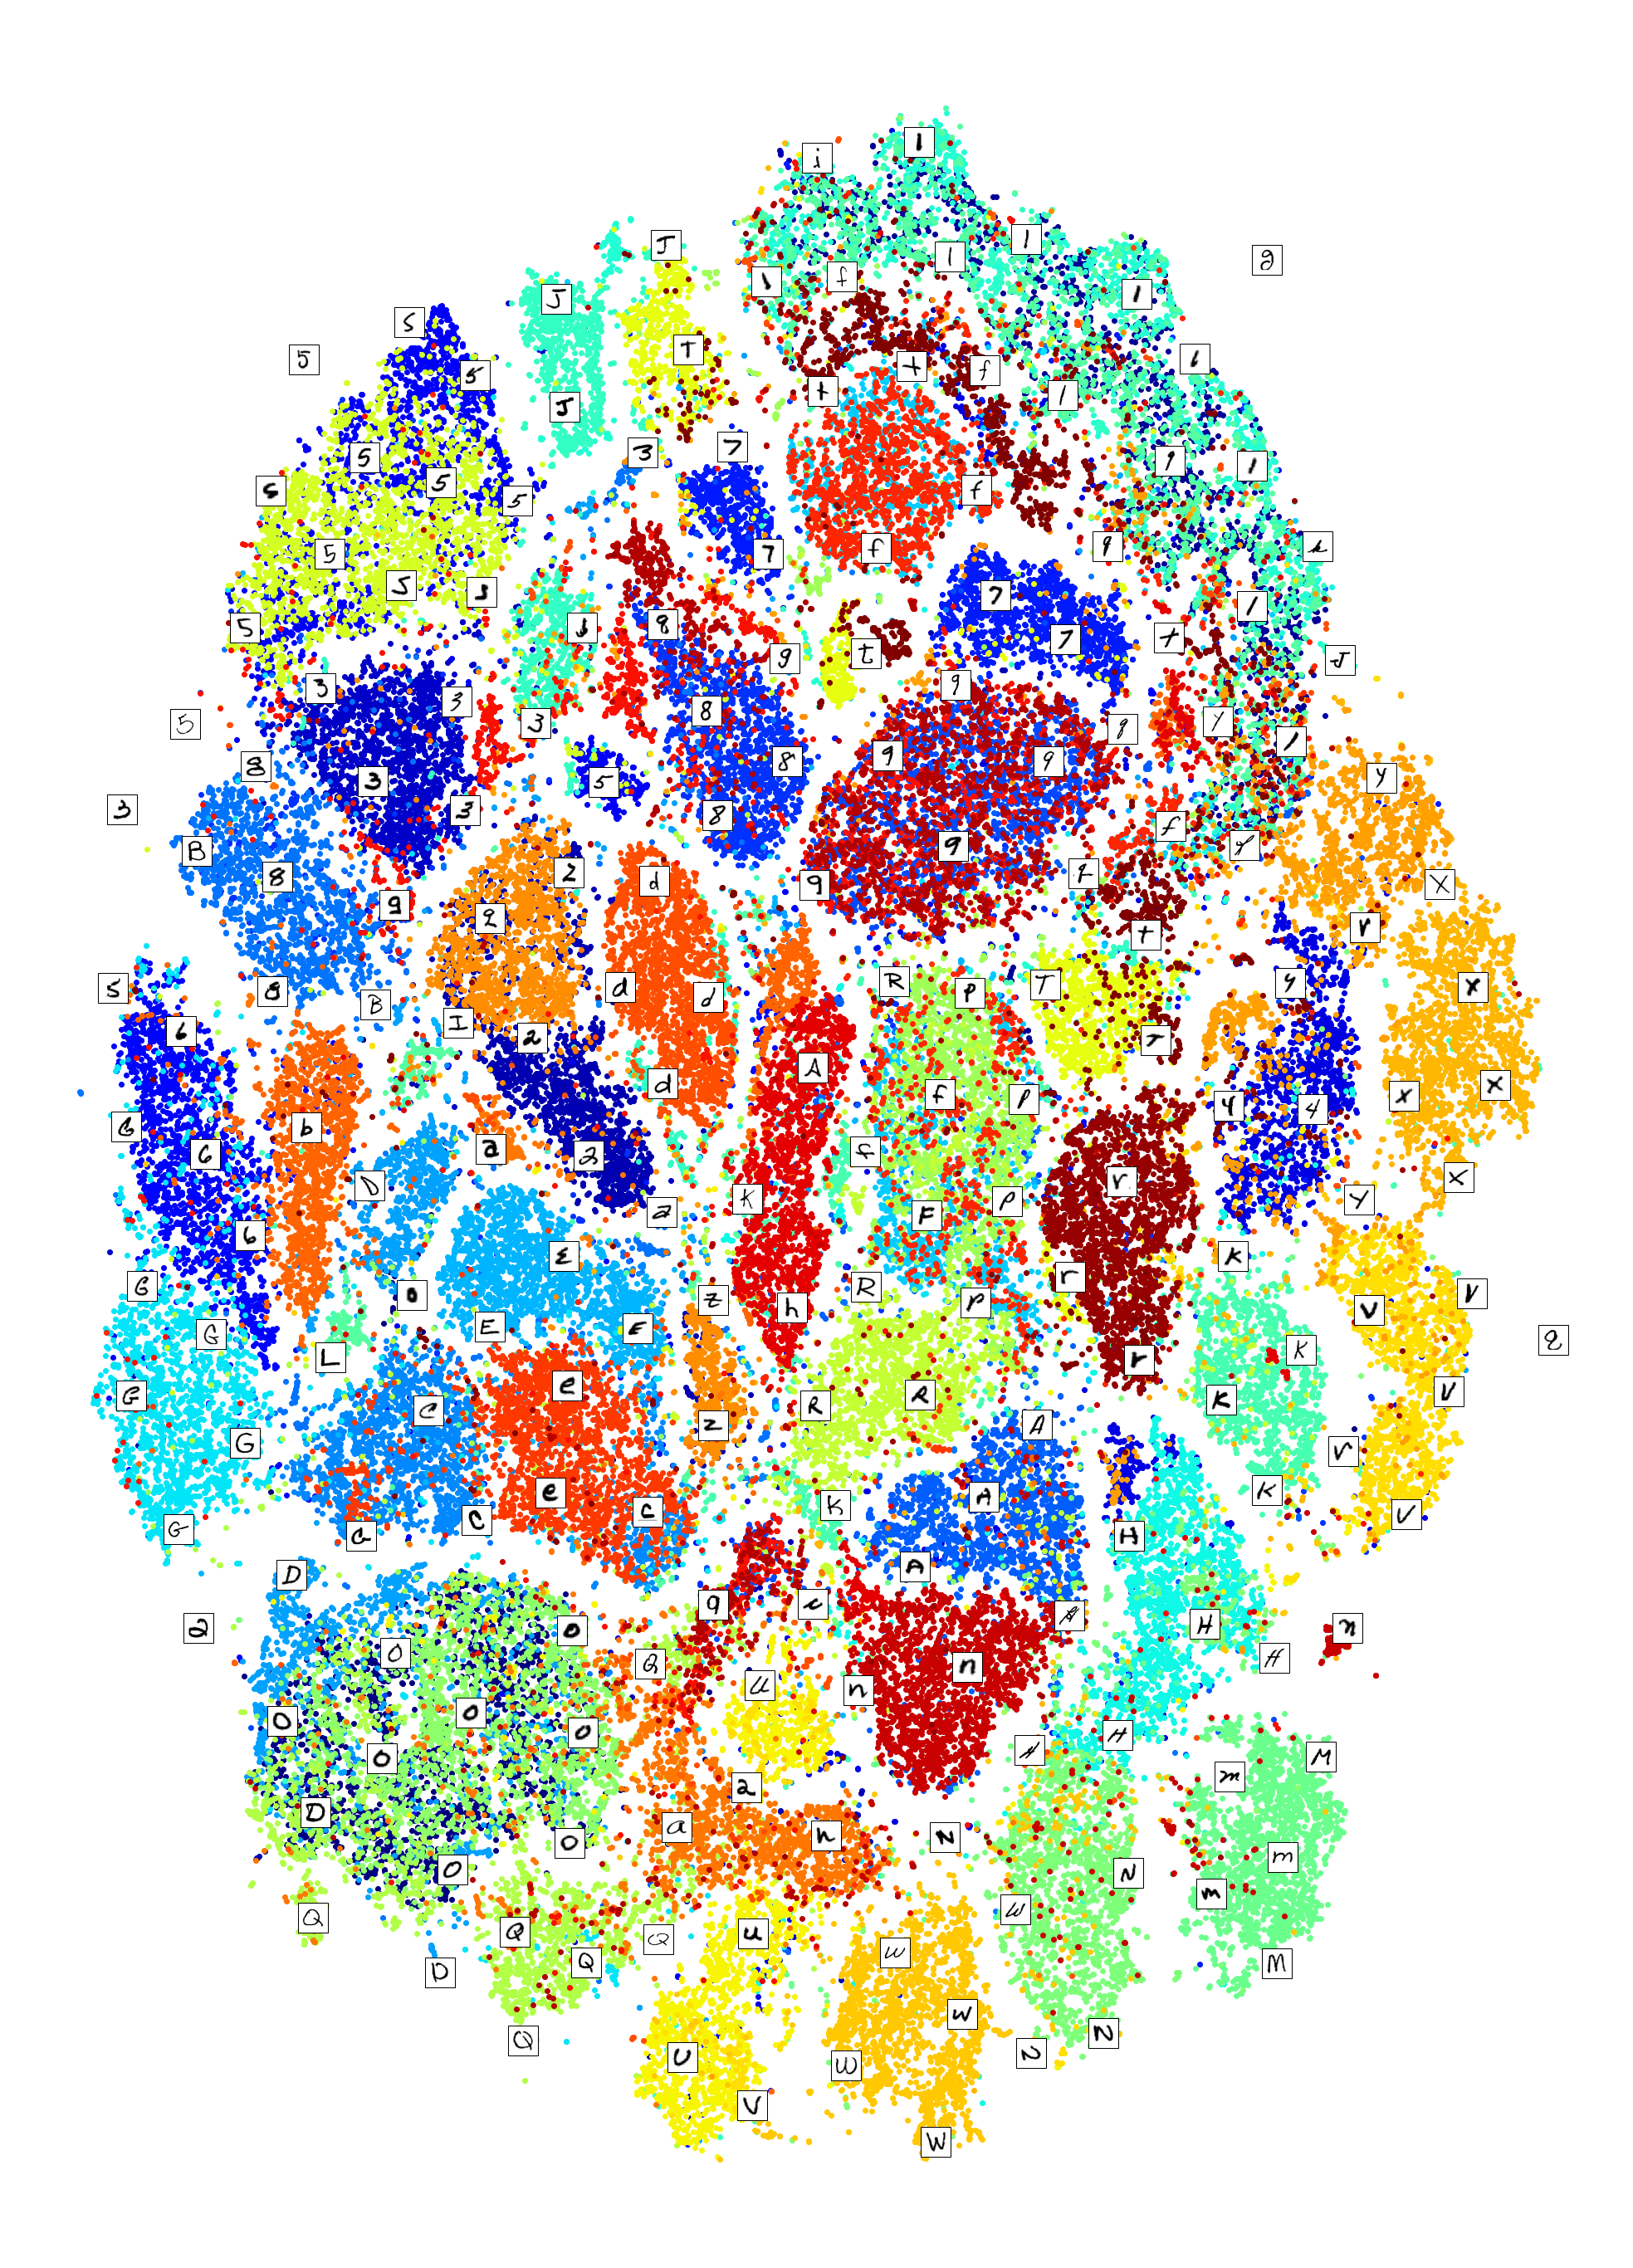
\includegraphics[width = 1\linewidth]{images/pca_tsne.png}
\captionof{figure}{Projecció PCA + t-SNE sobre les dades EMNIST balancejades}
\label{fig:pca_tsne}
\end{figure}

%%%

\begin{figure}[hbt!]
\centering
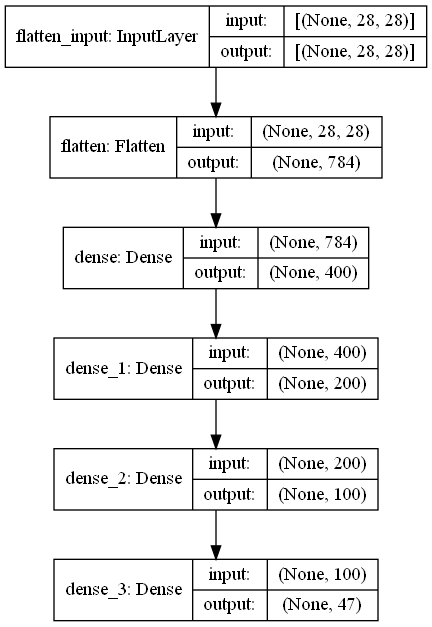
\includegraphics[width = 0.65\linewidth]{images/nn_estructure.png}
\captionof{figure}{Capes de la xarxa neuronal a modelitzar, amb el nombre de neurones per capa d'input i output.}
\label{fig:nn_estructure}
\end{figure}




% Fitxer bibliografia scibib.bib

\clearpage
\bibliography{scibib}

\bibliographystyle{Science}


% Citacions extra manuals

\begin{scilastnote}
\item Codi desenvolupat: \href{https://github.com/cesc1/TFG}{github/cesc1/TFG}

\end{scilastnote}


\end{document}




















